\newpage
%% PPS viene da: https://towardsdatascience.com/rip-correlation-introducing-the-predictive-power-score-3d90808b9598
\section{Feature Selection}\label{sec:featureselection}
After applying all the procedures described in the previous section,
we find ourselves with a dataset composed of 764 columns.
This high number of features would make it nearly impossible to train various models,
both from a purely hardware perspective and due to the excessive information redundancy.
In an attempt to minimize the number of features as much as possible,
we applied and combined the results of two essential tools for feature selection:
the \textit{Correlation Matrix} \cite{corr} and the \textit{Power Predictive Score} \cite{pps}.

%Dopo aver applicato tutte le procedure descritte nella precedente sezione,
%ci ritroviamo con un dataset formato da 764 colonne. Questo elevato
%numero di features renderebbe quasi impossibile l'allenamento dei vari
%modelli, sia dal punto di vista puramente hardware che per l'eccessiva 
%ridondanza delle informazioni. Per cercare di ridurre il più possibile
%il numero di features abbiamo applicato e unito i risultati di due
%strumenti fondamentali per la fearue selection: Correlation Matrix e Power Predictive Score.

\begin{figure}[H]
	\centering
	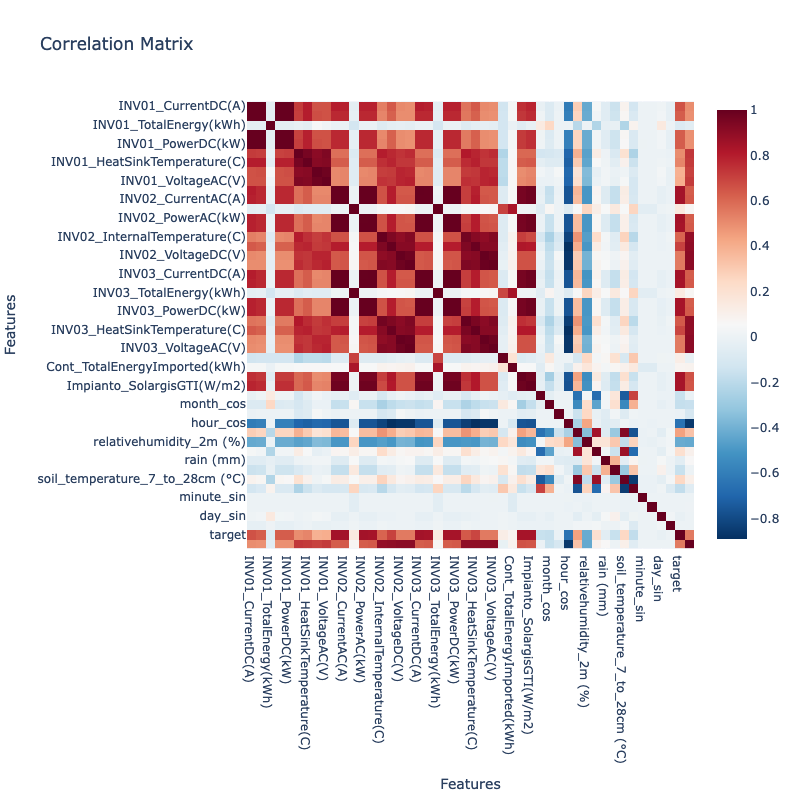
\includegraphics[width=\textwidth, keepaspectratio]{chapters/2_data_preprocessing/imgs/correlationmatrix.png}
	\caption{Correlation Matrix}\label{fig:corrmatrix}
\end{figure}
As we can infer, even with a naive approach, all the information from the various
String Boxes and Junction Boxes is perfectly summarized by the data provided by the
various Inverters (see Section~\ref{sec:pv}); a similar reasoning can be applied to the features
coming from \textit{Other} (those starting with \verb|other_|), as they do not provide any
useful information for energy estimation. Consulting the Correlation Matrix (Figure~\ref{fig:corrmatrix}), we can
see that this naive reasoning is confirmed because the features of the junction boxes
have a high level of correlation with those of the Inverters.
In general, we want to retain features that are minimally correlated with each other
and aim to discard highly correlated ones, keeping only those that are more representative.

%Come possiamo intuire, anche con un approccio naive, tutte  le informazioni delle varie String Box e Junction Box vengono riassunte perfettamente dai dati
%che ci forniscono i vari Inverter (vedi Sezione \ref{sec:pv}); un quasi simile
%ragionamento può essere fatto per le feature che provengono da \textit{Other} (quelle che iniziano con \verb|other_|) dato che non apportano nessuna
%informazione utile alla stima dell'energia.
%Consultando la Correlation Matrix possiamo vedere che questo ragionamento
%naive è confermato, in quanto le feature delle junction box hanno un alto
%tasso di correlazione rispetto a quelle degli Inverter. In generale,
%vogliamo tenere feature che sono poco correlate tra di loro e cercare di 
%scartare quelle molto correlate tenendone solo alcune che sono più 
%rappresentative.
Applying this approach straightforwardly, however, is not the best choice because it
could lead to the loss of important information.
Let's consider an example: let's take into account the features \verb|INV01_Power(kW)|,
\verb|INV02_Power(kW)|, and \verb|INV03_Power(kW)|; by examining the correlation matrix, these
three features are highly correlated, and, therefore, we should retain only one of them.
However, all three are important for predicting our target.
For instance, if Inverter 1 experiences any issues and is not operating at 100\%,
this will impact the total energy production, making all three of these
features indispensable. Therefore, in conjunction with the correlation matrix,
we have utilized the \textit{Power Predictive Score} (PPS): an asymmetric,
data-type-agnostic score that can detect linear or non-linear relationships
between two or more columns \cite{pps}. The score ranges from 0 (no predictive power)
to 1 (perfect predictive power) \cite{pps}.

%Applicare questo approccio in modo straight forward non è però la scelta migliore,
%in quanto potrebbe farci perdere informazioni importanti.
%Facciamo un esempio: prendiamo in considerazione le features \verb|INV01_Power(kW)|, \verb|INV02_Power(kW)| e \verb|INV03_Power(kW)|;
%controllando la matrice di correlazione queste 3 risutano estremamente correlate
%e quindi ne dovremmo tenere soltanto una, ma tutte e 3 risultano importanti
%ai fini della predizione del nostro target: se, per esempio, l'Inverter 1 ha
%avuto qualche problema e non è operativo al 100\% questo si va a riflettere
%sull'energia totale prodotta, rendendo queste feature tutte e 3 indispensabili.
%Abbiamo quindi utilizzato in concomitanza alla matrice di correlazione il \textit{Power Predictive Score} (PPS): an asymmetric, data-type-agnostic
%score that can detect linear or non-linear relationships between two or more columns.
%The score ranges from 0 (no predictive power) to 1 (perfect predictive power).
%
\begin{figure}[H]
	\centering
	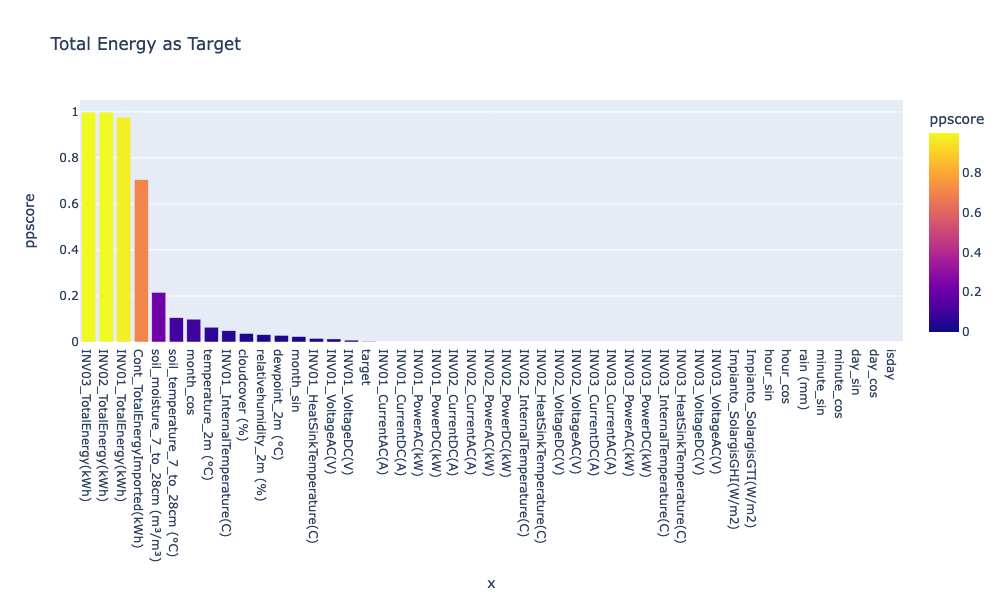
\includegraphics[width=.9\textwidth, keepaspectratio]{chapters/2_data_preprocessing/imgs/ppcontottenergy.png}
	\caption{All features PPS using \texttt{Cont\_TotalEnergy(kWh)} as target.}\label{fig:ppsTotEnergy}
\end{figure}


\begin{figure}[H]
	\centering
	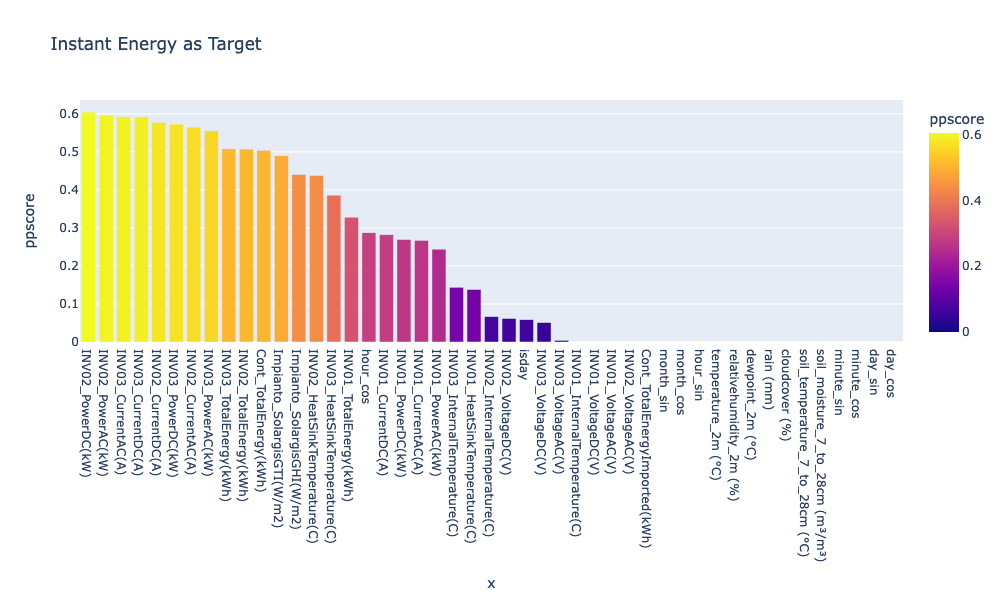
\includegraphics[width=.9\textwidth, keepaspectratio]{chapters/2_data_preprocessing/imgs/pptarget.png}
	\caption{All feature PPS using Instant Energy (\texttt{target}) as Target.}\label{fig:ppstarget}
\end{figure}

As we can see in Figures~\ref{fig:ppsTotEnergy} and \ref{fig:ppstarget}, the features
that perform better in predicting the instantaneous energy production trend are
indeed those of the Inverters, confirming the reasoning described earlier.
Finally, by combining the results obtained from the Correlation Matrix and the
Power Predictive Score, we obtain a final set of 33 features.

%Come possiamo vedere nelle Figure \ref{fig:ppsTotEnergy} e \ref{fig:ppstarget}
%le feature che riescono meglio a predirre l'andamento dell'energia istananea
%prodotta sono proprio quelle degli Inverter, confermando quindi il ragionamento
%descritto prima.
%Infine, combinando i risultati ottenuti dalla Correlation Matrix e dal PPS,
%otteniamo un set finale di 28 features.
%
\begin{table}[H]
	\begin{center}
		\begin{tabular}[t]{l|}
			\verb|INV01_PowerAC(kW)|      \\
			\verb|INV01_PowerDC(kW)|      \\
			\verb|INV02_PowerAC(kW)|      \\
			\verb|INV02_PowerDC(kW)|      \\
			\verb|INV03_PowerAC(kW)|      \\
			\verb|INV03_PowerDC(kW)|      \\
			\verb|INV01_CurrentAC(A)|     \\
			\verb|INV01_CurrentDC(A)|     \\
			\verb|INV02_CurrentAC(A)|     \\
			\verb|INV02_CurrentDC(A)|     \\
			\verb|INV03_CurrentAC(A)|     \\
			\verb|INV03_CurrentDC(A)|     \\
			\verb|INV01_TotalEnergy(kWh)| \\
			\verb|INV02_TotalEnergy(kWh)|
		\end{tabular}
		\begin{tabular}[t]{l|}
			\verb|INV03_TotalEnergy(kWh)|       \\
			\verb|INV01_HeatSinkTemperature(C)| \\
			\verb|INV02_HeatSinkTemperature(C)| \\
			\verb|INV03_HeatSinkTemperature(C)| \\
			\verb|Impianto_SolargisGHI(W/m2)|   \\
			\verb|Impianto_SolargisGTI(W/m2)|   \\
			\verb|Cont_TotalEnergy(kWh)|        \\
			\verb|rain (mm)|                    \\
			\verb|cloudcover (%)|               \\
			\verb|hour_sin|                     \\
			\verb|hour_cos|                     \\
			\verb|day_sin|                      \\
			\verb|day_cos|                      \\
			\verb|month_sin|
		\end{tabular}
		\begin{tabular}[t]{l}
			\verb|month_cos| \\
			\verb|min_sin|   \\
			\verb|min_cos|   \\
			\verb|target|    \\
			\verb|is_day|
		\end{tabular}
	\end{center}
	\caption{All feature selected after this phase.}\label{tab:featselected}
\end{table}


%\begin{figure}[H]
%    \centering
%        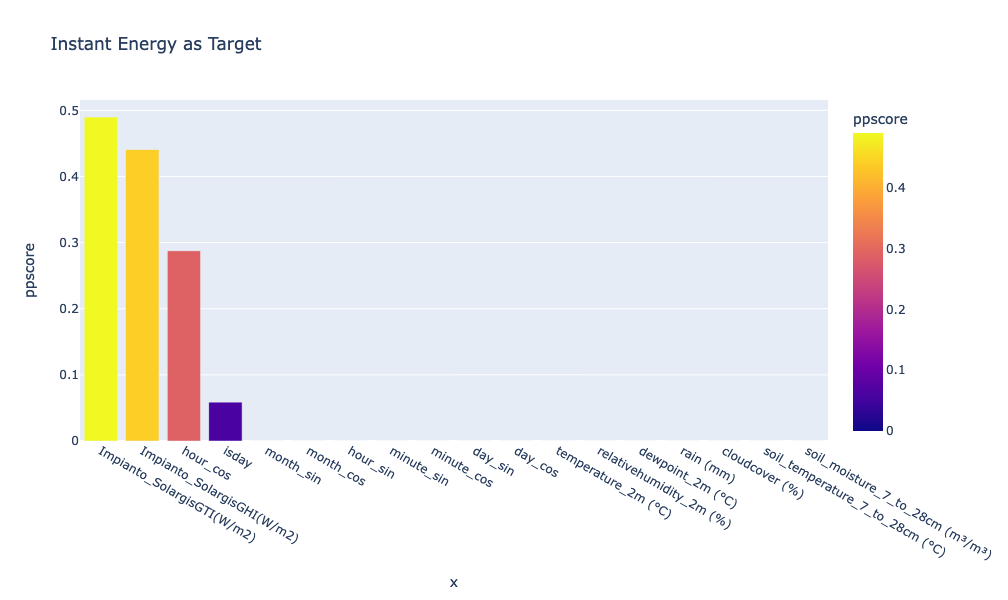
\includegraphics[width=\textwidth, keepaspectratio]{chapters/2_data_preprocessing/imgs/ppbucotarget.png}
%    \caption{Only Wather features PPS using Instant Energy (\texttt{target}) as Target.}
%    \label{fig:ppssolargis}
%\end{figure}